\documentclass[border=2mm]{standalone}
\usepackage{tikz}
\begin{document}
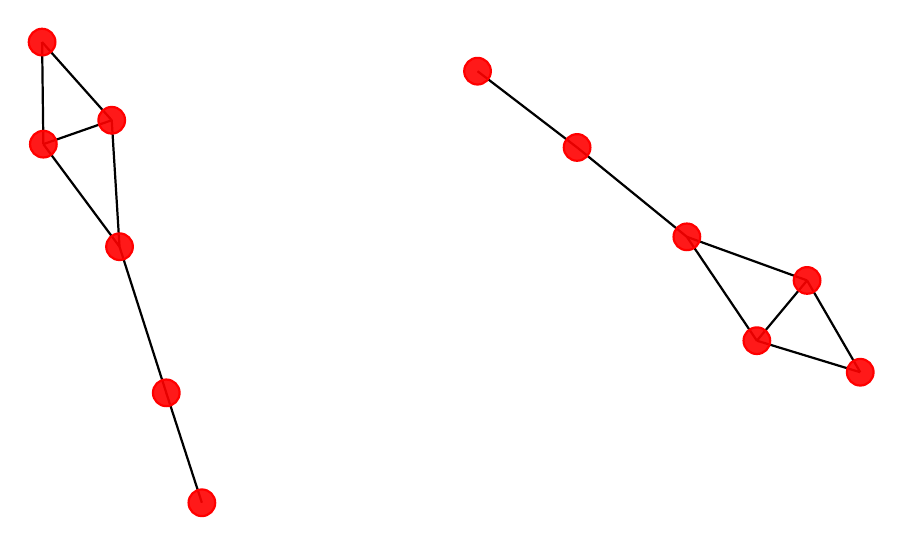
\begin{tikzpicture}[line width=0.5pt,fill opacity=0.9,scale = 3.5]
\tikzstyle{every path}=[draw, thick]
\tikzstyle{every node}=[draw, circle, fill=red, inner sep=3.4pt]
\coordinate (v_0) at (1.00000, 0.72335) {};
\coordinate (v_4) at (1.00459, 0.35303) {};
\coordinate (v_5) at (1.57969, -0.94799) {};
\coordinate (v_8) at (1.25261, 0.43977) {};
\coordinate (v_9) at (1.28095, -0.01905) {};
\coordinate (v_10) at (1.45051, -0.54912) {};
\coordinate (v_1) at (3.96818, -0.47438) {};
\coordinate (v_2) at (3.59311, -0.35997) {};
\coordinate (v_3) at (2.57969, 0.61776) {};
\coordinate (v_6) at (3.33915, 0.01682) {};
\coordinate (v_7) at (2.94095, 0.34111) {};
\coordinate (v_11) at (3.77530, -0.14134) {};
\path (v_0) -- (v_4);
\path (v_0) -- (v_8);
\path (v_1) -- (v_2);
\path (v_1) -- (v_11);
\path (v_2) -- (v_6);
\path (v_2) -- (v_11);
\path (v_3) -- (v_7);
\path (v_4) -- (v_8);
\path (v_4) -- (v_9);
\path (v_5) -- (v_10);
\path (v_6) -- (v_7);
\path (v_6) -- (v_11);
\path (v_8) -- (v_9);
\path (v_9) -- (v_10);
\node[red] (x_0) at (v_0) {};
\node[red] (x_4) at (v_4) {};
\node[red] (x_5) at (v_5) {};
\node[red] (x_8) at (v_8) {};
\node[red] (x_9) at (v_9) {};
\node[red] (x_10) at (v_10) {};
\node[red] (x_1) at (v_1) {};
\node[red] (x_2) at (v_2) {};
\node[red] (x_3) at (v_3) {};
\node[red] (x_6) at (v_6) {};
\node[red] (x_7) at (v_7) {};
\node[red] (x_11) at (v_11) {};
\end{tikzpicture}
\end{document}
